\documentclass[10pt, a4paper]{article}
	% 使用12pt(对应于中文的小四号字)
	% \usepackage{xeCJK} 
	% \setmainfont{Times New Roman} 
	% \setCJKmainfont[BoldFont=Hei]{Hei} 
    \usepackage{array, ragged2e, pst-node, pst-dbicons}
	\usepackage{ctex}
	\usepackage{geometry}   %设置页边距的宏包
    \usepackage{titlesec}   %设置页眉页脚的宏包
    \usepackage{amssymb}
    \usepackage{amsmath}
    \usepackage{tikz-er2}
	\usepackage{graphviz}
	\usepackage{minted}
	\usepackage[utf8]{inputenc}
	\usepackage{tikz}
	\usetikzlibrary{automata, positioning, arrows, shapes.geometric}

	\tikzstyle{startstop} = [rectangle, rounded corners, minimum width=3cm, minimum height=1cm,text centered, draw=black, fill=red!30]
	\tikzstyle{io} = [trapezium, trapezium left angle=70, trapezium right angle=110, minimum width=3cm, minimum height=1cm, text centered, draw=black, fill=blue!30]
	\tikzstyle{process} = [rectangle, minimum width=3cm, minimum height=1cm, text centered, draw=black, fill=orange!30]
	\tikzstyle{decision} = [diamond, minimum width=3cm, minimum height=1cm, text centered, draw=black, fill=green!30]
	\tikzstyle{arrow} = [thick,->,>=stealth]
	\newminted{text}{frame=lines, framesep=2mm}
	\newminted{python}{frame=lines,  framesep=2mm,  linenos}
    \geometry{left=3.17cm, right=3.17cm, top=2.54cm, bottom=2.54cm}  %设置 上、左、下、右 页边距
	\begin{document}
	\newpagestyle{main}{            
		\sethead{哈尔滨工业大学}{数据库系统\_第六次作业}{1160300314 朱明彦}     %设置页眉
		% \setfoot{左页脚}{中页脚}{右页脚}      %设置页脚, 可以在页脚添加 \thepage  显示页数
		\setfoot{}{}{\thepage}
		\headrule                                      % 添加页眉的下划线
		% \footrule                                       %添加页脚的下划线
	}
	\pagestyle{main}    %使用该style
	\usetikzlibrary{positioning}
	\usetikzlibrary{shadows}
	\usetikzlibrary{arrows}
	\tikzstyle{every entity} = [top color=white,  bottom color=blue!30,  
                            draw=blue!50!black!100,  drop shadow]
	\tikzstyle{every weak entity} = [drop shadow={shadow xshift=.7ex,  
                                 shadow yshift=-.7ex}]
	\tikzstyle{every attribute} = [top color=white,  bottom color=yellow!20,  
                               draw=yellow,  node distance=1cm,  drop shadow]
	\tikzstyle{every relationship} = [top color=white,  bottom color=red!20,  
                                  draw=red!50!black!100,  drop shadow]
	\tikzstyle{every isa} = [top color=white,  bottom color=green!20,  
                         draw=green!50!black!100,  drop shadow]

	% \setlength{\baselineskip}{15.6pt}
	% \setlength{\parskip}{0pt}
	\renewcommand{\baselinestretch}{1.5}
	
	\begin{enumerate}
		\item \begin{enumerate}
			\item \textbf{选择PlanA。}理由是,一般情况下优先做选择($\sigma$)操作可以减少用于连接元组的数量,进一步降低连接的代价。
			\item \textbf{是。}理由是,如果已知$R$和$S$在连接属性值$k$上的分布,并且二者没有交集。
		\end{enumerate}
		\item 可以画出原有调度的优先图如图\ref{fig:2},从图中可以看到在$0$和$2$中存在环路,所以\textbf{这不是一个冲突可串行化调度}。
		\begin{figure}[htb]
			\centering
			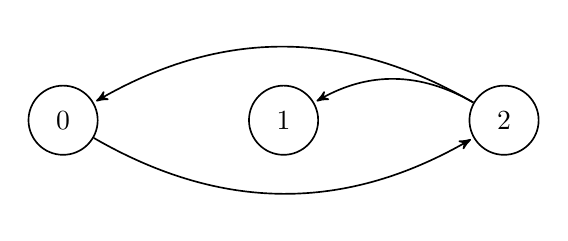
\begin{tikzpicture}[->,>=stealth',shorten >=1pt,auto,node distance=2.8cm,semithick]
				\node[state] (q0) {$0$};
				\node[state, right of=q0] (q1) {$1$};
				\node[state, right of=q1] (q2) {$2$};
				\draw (q0) edge [bend right, above] (q2)
					(q2) edge [bend right, above] (q0)
					(q2) edge [bend right, above] (q1);
			\end{tikzpicture}
			\caption{第2题调度的优先图}
			\label{fig:2}
		\end{figure}
		\item 用两阶段锁保证题目2的调度冲突可并行化,\textbf{结果如表\ref{tab:3}所示}。
		\begin{table}[htb]
			\centering
			\begin{tabular}{l|l|l}
			T0    & T1    & T2    \\ \hline
			\textbf{LOCK-X(A)} & &\\
			r0(A) &       &       \\ 
			w0(A) &       & 	  \\
			\textbf{LOCK-X(B)}& & \\ 
			r0(B) &       &       \\
			w0(B) &       &       \\ 
			\textbf{UNLOCK(A)} & &\\
			& & \textbf{LOCK-X(A)}\\
			\textbf{UNLOCK(B)} & &\\
			& & w2(A) \\
			& & r2(A) \\ 
			& & \textbf{LOCK-X(B)}\\ 
			& & r2(B) \\ 
			& & W2(B) \\
			& & \textbf{UNLCOK(A)}\\
			&\textbf{LOCK-S(A)}&  \\
			& & \textbf{UNLOCK(B)}\\ 
				  & r1(A) &       \\
				  &\textbf{LOCK-S(B)} & \\
				  & r1(B) &       \\
			& \textbf{UNLOCK(A)} &\\
			& \textbf{UNLOCK(B)} &\\ 
			\end{tabular}
			\caption{使用两阶段锁保证调度的冲突可并行化}\label{tab:3}
			\end{table}
		\item \textbf{结果如表\ref{tab:4}所示},其中在T2执行完Write(A)时,由于TS(T2) $<$ R-ts(A),所以T2需要回滚。
		\begin{table}[htb]
			\centering
			\begin{tabular}{|l|l|l|l|l|l|}
			\hline
			T1            & T2            & W-ts(A) & R-ts(A)         & W-ts(B)         & R-ts(B)         \\ \hline
						  & Read(B);      &         &                 & \textbf{}       & \textbf{TS(T2)} \\ \hline
						  & B := B - 50;  &         &                 & \textbf{}       & \textbf{TS(T2)} \\ \hline
						  & Write(B);     &         &                 & \textbf{TS(T2)} & \textbf{TS(T2)} \\ \hline
			READ(B);      &               &         &                 & \textbf{TS(T2)} & \textbf{TS(T1)} \\ \hline
						  & READ(A);      &         & \textbf{TS(T2)} & \textbf{TS(T2)} & \textbf{TS(T1)} \\ \hline
						  & A := A = 50;  &         & \textbf{TS(T2)} & \textbf{TS(T2)} & \textbf{TS(T1)} \\ \hline
			Read(A);      &               &         & \textbf{TS(T1)} & \textbf{TS(T2)} & \textbf{TS(T1)} \\ \hline
						  & Write(A);     & 出现错误 & \textbf{TS(T1)} & \textbf{TS(T2)} & \textbf{TS(T1)} \\ \hline
			Display(A+B); &               &         & \textbf{TS(T1)} & \textbf{TS(T2)} & \textbf{TS(T1)} \\ \hline
						  & Display(A+B); &         & \textbf{TS(T1)} & \textbf{TS(T2)} & \textbf{TS(T1)} \\ \hline
			\end{tabular}
			\caption{时间戳}\label{tab:4}
			\end{table}
		\item \begin{enumerate}
			\item \textbf{结果如表\ref{tab:5_a}所示。}
			\begin{table}[htb]
				\centering
				\begin{tabular}{|l|l|}
				\hline
				1  & \textbf{\textless{}T0,start\textgreater{}}         \\ \hline
				2  & \textless{}T0, A, 50, 70\textgreater{}             \\ \hline
				3  & \textbf{\textless{}T2,start\textgreater{}}         \\ \hline
				4  & \textless{}start checkpoint (T0, T2)\textgreater{} \\ \hline
				5  & \textless{}end checkpoint\textgreater{}            \\ \hline
				6  & \textless{}T1, commit\textgreater{}                \\ \hline
				7  & \textbf{\textless{}T1, B, 30, 20\textgreater{}}    \\ \hline
				8  & \textless{}T1, commit\textgreater{}                \\ \hline
				9  & \textless{}T2, C, 35, 70\textgreater{}             \\ \hline
				10 & \textbf{\textless{}T3, start\textgreater{}}        \\ \hline
				11 & \textless{}T3, D, 15, 30\textgreater{}             \\ \hline
				12 & \textbf{\textless{}T2, commit\textgreater{}}       \\ \hline
				\end{tabular}
				\caption{日志文件}\label{tab:5_a}
				\end{table}
			\item \textbf{T1和T2需要Redo,T3和T0需要Undo}。根据日志文件,在故障恢复时T1和T2已经提交,需要Redo;而T0和T3未提交故Undo,需要消除其影响。
			\item \textbf{需要增加<T0, A, 50>,<T0, abort>和<T3, D 15><T3, abort>},表明T0和T3在故障中终止未提交。
		\end{enumerate}
	\end{enumerate}
\end{document}